\documentclass[12pt,a4paper]{article}

\usepackage[latin1]{inputenc}
\usepackage{geometry}
\geometry{a4paper,left=30mm,right=30mm, top=25mm, bottom=25mm} 
\usepackage{setspace}
%\setstretch{1,1666} %entspricht 14pt Zeilenabstand bei 11er Schrift = 14/11
\usepackage{datetime}
\usepackage[numbers]{natbib}
\usepackage{amsmath}
\usepackage{sistyle}
\usepackage{amsfonts}
\usepackage{amssymb}
\usepackage{graphicx}
%\usepackage[linkcolor=blue,urlcolor=blue]{hyperref}
\usepackage{lineno}
\usepackage{textcomp}
\usepackage{booktabs}
\usepackage{fontawesome} % die runden Symbole Phone Email etc. 
\usepackage{markdown}
\usepackage{marvosym} % F�r das HandySymbol auf dem Deckblatt

\usepackage{tikz}
\usetikzlibrary{patterns}

%%%% Korrekte Darstellung von Datum und Zeit
\usepackage[german]{babel}
\usepackage{datetime}



%%% ToDo Notes
%\usepackage[
%linecolor=orange,
%backgroundcolor=white,
%bordercolor=orange,
%textsize=tiny]{todonotes}

\usepackage{natbib} %Author Year
%\usepackage[numbers]{natbib}




\usepackage{hyperref}
\hypersetup
{
	colorlinks=true,
	linkcolor=blue,
	filecolor=magenta,      
	urlcolor=blue,
	citecolor=blue,
	%bookmarks=true,
	bookmarksopen=true,
	bookmarksnumbered=true,
	urlbordercolor={1 0 0},
	linkbordercolor={1 0 0},
	pdftitle={LTC - Assignment Winter 20-21},
	%pdfauthor={},
	pdfstartpage=1,
	%pdftoolbar=false,
	%pdfmenubar=false,
	pdfdisplaydoctitle=true,
}
\newcommand{\assignment}{Assignment 1}
\newcommand{\topic}{2D Kinematik beim Weitsprung}
\newcommand{\group}{Gruppe 4711}
\newcommand{\lastcompile}{\today \hspace{0.25cm}\currenttime}
	
\begin{document}

%%%%%% ZEILENNUMMERN %%%%%%%
\linenumbers % Einschalten der Zeilennummern
\modulolinenumbers[5] % Jede fuenfte Zeile 
\setlength\linenumbersep{1cm} % Abstand zwischen Zahl und Text


% Hier kommt die Titelseite via Input rein
\thispagestyle{empty}
\vspace*{3cm}
\begin{center}
\hrulefill \\
{\Large  \textbf{\assignment \\ \topic \\ \group} \par}
\hrulefill \\ \lastcompile
\end{center}
\vfill
\textbf{Dozierender:}\\
Dr. Bj\"orn Braunstein\\
\faPhone \hspace{5pt} +49.(0)221.4982.5621\\
\faEnvelopeO \hspace{5pt} braunstein@dshs-koeln.de\\[14pt]
\noindent
\textbf{Kontaktperson:}\\
BA Sc. Vorname Nachname\\
%\faPhone \hspace{5pt} +49.(0)221.4982.5621\\
\faEnvelopeO \hspace{5pt} info@info.de\\
Matrikelnummer: 08154711\\[14pt]
\noindent
\textbf{Mitstreiter:}\\
Vorname Nachname (ID: 08154711)\\
Vorname Nachname (ID: 08154711)\\
Vorname Nachname (ID: 08154711)\\
Vorname Nachname (ID: 08154711)\\
Vorname Nachname (ID: 08154711)

 


\newpage
\section{Theoretisches Basiswissen} \label{ch:theorie}
Rope Skipping (RS) (Abb.:\ref{fig:Seilchenspringer}) has been a common leisure-time activity of children for generations \cite{gowitzke1989}. Today, especially Asia holds high popularity of rope skippers with 87.4\% of the Chinese youth participating in jump rope exercises at least once a week \cite{Li2013}. Defined as a repetitive vertical jump with both feet losing contact to the ground to allow rope rotation \cite{gowitzke1989}, RS can be performed both outdoors and indoors by using inexpensive equipment \cite{wong2004}.\\
\begin{figure} [h] \centering
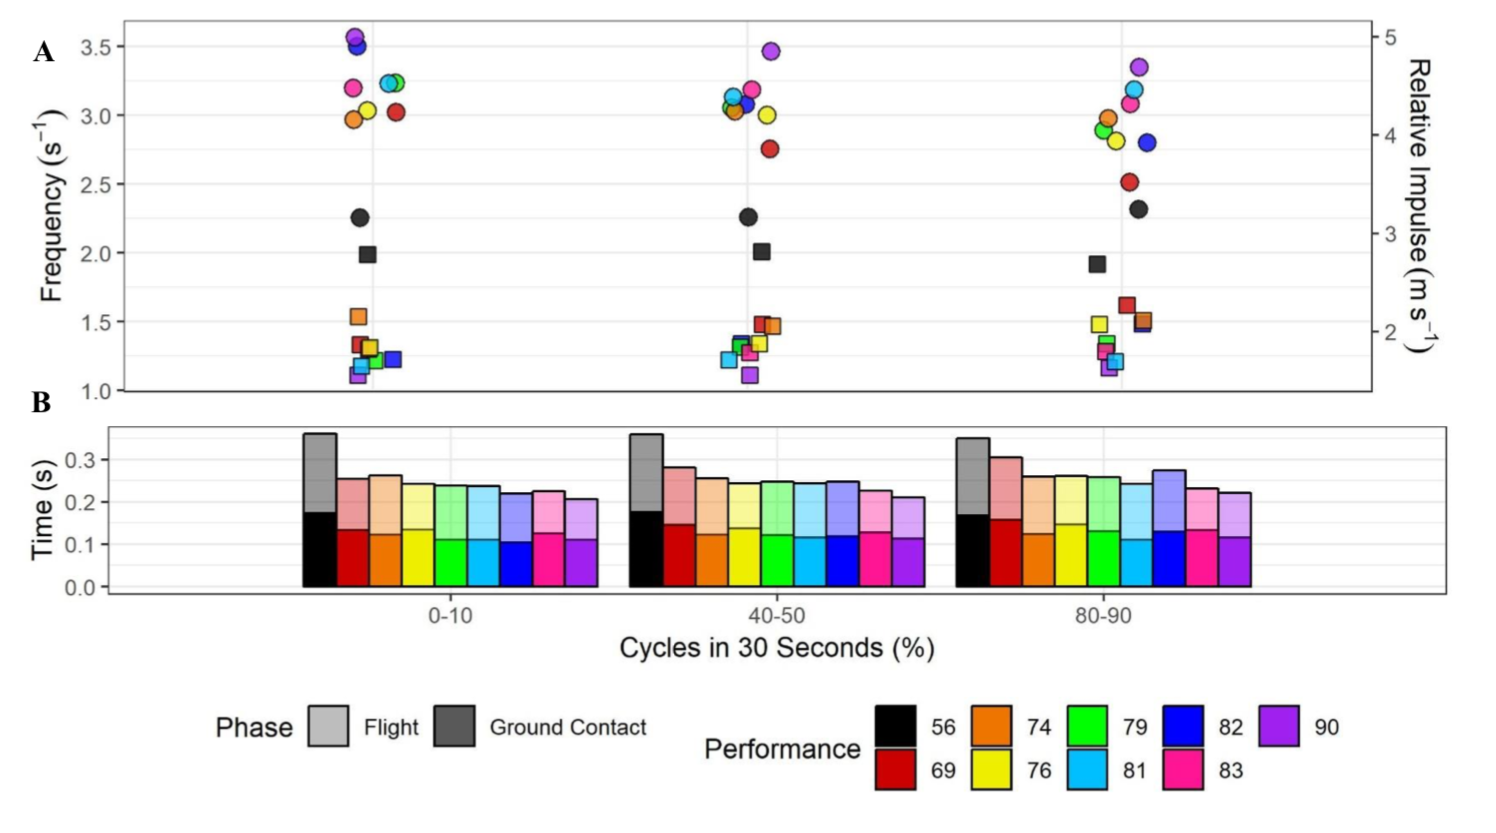
\includegraphics[width=0.9\textwidth]{pix/fig3.png}
    \caption{Hier steht dann die korrekte Beschreibung vom Bild manchmal sogar direkt mit einer Referenz \cite{Li2013}}
    \label{fig:Seilchenspringer}
\end{figure}


\newpage
\section{Anwendungsorietierter Teil} \label{ch:praxis}
\subsection{Subjects}
This study was conducted with the formal approval of the university ethics committee (\textnumero 137/2018) . All participants were informed about the experimental procedure together with potential risk factors and provided written informed consent to participate in this study. Descriptive data, including participants' anthropometrics, length and mass of their jump rope as well as athletes' personal best were collected prior to testing and are presented together with further group characteristics in Table \ref{tab:anthropo}.


\begin{table}[h!]\centering
    \caption{Der Beschreibungstext f\"ur Tabellen nat\"urlich immer dr\"uber} \vspace{1ex}
    \begin{tabular}{lcccc}
    \toprule
    \textbf{Subj. ID} & \textbf{Gender} & \textbf{Height} & \textbf{Mass} & \textbf{Skills}\\
    Matrikel & f/m & [cm] & [kg] & [1-6]\\
    \midrule
    4711 & f& 186&84& 2\\
    0815 & m&176&76 & 3\\
    4711 & f& 186&84& 2\\
    0815 & m&176&76 & 3\\
    4711 & f& 186&84& 2\\
    0815 & m&176&76 & 3\\
    4711 & f& 186&84& 2\\
    0815 & m&176&76 & 3\\
    \bottomrule
    \end{tabular}
    \label{tab:anthropo}
\end{table}

\newpage
\section{markdown} \label{ch:markdown}
\begin{markdown}
I'm a markdown.  
And I can do *emphasis*.

## With sub-headers

> 'Block quotes are
> written like so.'
>
> 'They can span multiple paragraphs,
> if you like.'

Hier dann irgend ein Text

* this one
* that one
* the other one

\end{markdown}

\vspace{1cm}
\href{https://www.overleaf.com/learn/how-to/Writing_Markdown_in_LaTeX_Documents}{Hier kann man sich dann auch weiter austoben durch klicken}



\newpage
\bibliography{lit/lit}
\bibliographystyle{plainnat}
%\bibliographystyle{abbrvdin}
%\bibliographystyle{unsrtnat}
%\bibliographystyle{abbrv}


\end{document}